\documentclass{standalone}
\usepackage{tikz}
\usetikzlibrary{circuits.logic.US}
\usetikzlibrary{positioning}

\begin{document}
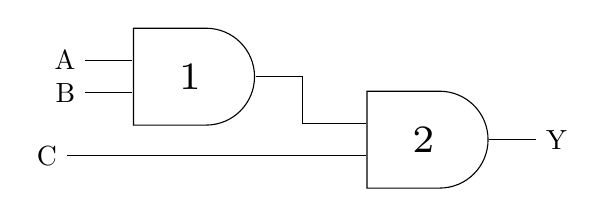
\begin{tikzpicture}[circuit logic US, scale=2]
	 \node [and gate, inputs=nn] (lg1) {\scriptsize 1};
	 \node [and gate, inputs=nn, right=of lg1, xshift=-3mm, yshift=-4mm] (lg2) {\scriptsize 2};
	 \draw (lg1.output) -- ++(right:3mm) |- (lg2.input 1);
	 \draw (lg1.input 1) -- node[at end,left]{A} ++(left:3mm);
	 \draw (lg1.input 2) -- node[at end,left]{B} ++(left:3mm);
	 \draw (lg2.input 2) -- node[at end,left]{C} ++(left:19mm);
	 \draw (lg2.output) -- node[at end,right]{Y} ++(right:3mm);
 \end{tikzpicture}
\end{document}